\section{Motivation and Scope}

There has been a strong desire for a more space- and/or runtime-efficient
representation for \code{map} among C++ users for some time now.  This has
motivated discussions among the members of SG14 resulting in a
paper\footnote{See P0038R0,
  \href{http://www.open-std.org/jtc1/sc22/wg21/docs/papers/2015/p0038r0.html}{here}.},
numerous articles and talks, and an implementation in Boost,
\code{boost::container::flat_map}\footnote{Part of Boost.Container,
  \href{http://www.boost.org/doc/libs/1_61_0/doc/html/container.html}{here}.}.
Virtually everyone who makes games, embedded, or system software in C++ uses
the Boost implementation or one that they rolled themselves.\\

Here are some numbers that show why.  The graphs that follow show runtimes for
different \code{map}-like associative containers.  The containers used are
Boost.FlatMap, \code{map}, and two thin wrappers over a sorted \code{vector};
the ``custom pair'' version of the sorted \code{vector} uses a simple
\code{struct} instead of \code{pair} for its value type.  All containers use
an \code{int} as the key type and an \code{int} or a \code{struct} with 5
\code{double}s for the value type.\\

All the graphs below were produced on Windows with MSVC 2015.  Similar results
were obtained on Linux, with Clang 3.9 and libc++, and with g++ 4.8.4 and
libstdc++.\\

These first four graphs cover the \code{int}-value-type case.  The first graph
shows insertion of N elements with random keys; the second shows full
iteration across all N elements; the third shows \code{map.lower_bound()}
called once for each key used in the original insertions; and the fourth shows
erasure of all N elements, by the keys used in the original insertions.

\begin{center}
    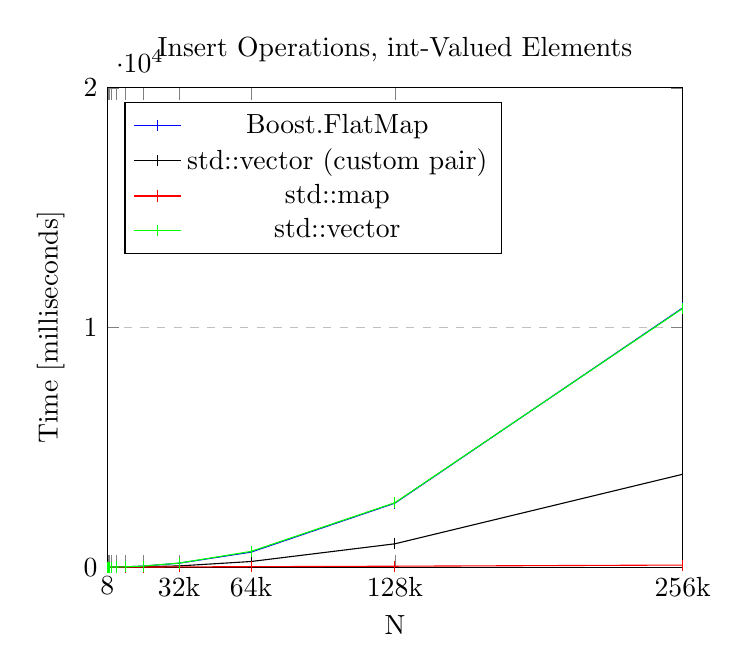
\begin{tikzpicture}
    \begin{axis}[
        width=3.5in,
        title={Insert Operations, int-Valued Elements},
        xlabel={N},
        ylabel={Time [milliseconds]},
        xmin=0, xmax=262144,
        ymin=0, ymax=20000.0,
        xtick={8,16,32,64,128,256,512,1024,2048,4096,8192,16384,32768,65536,131072,262144,524288},
        xticklabels={8,,,,,,,,,,,,32k,64k,128k,256k,512k},
        ytick={0.0,10000.0,20000.0,30000.0},
        legend pos=north west,
        ymajorgrids=true,
        grid style=dashed,
        scaled x ticks=false,
        scaled y ticks=true,
        legend entries={Boost.FlatMap,std::vector (custom pair),std::map,std::vector},
        ]

    \addplot[color=blue,mark=|,]
        coordinates {(8,0.0008412)(16,0.0016826)(32,0.003486)(64,0.0096148)(128,0.0170056)(256,0.0361772)(512,0.0998156)(1024,0.252279)(2048,0.834404)(4096,2.64516)(8192,10.8953)(16384,42.4244)(32768,162.432)(65536,625.67)(131072,2667.98)(262144,10816.6)};

    \addplot[color=black,mark=|,]
        coordinates {(8,0.0010214)(16,0.0018628)(32,0.003786)(64,0.0066108)(128,0.0133432)(256,0.0305282)(512,0.0712106)(1024,0.152699)(2048,0.443251)(4096,1.39556)(8192,3.84331)(16384,14.3052)(32768,49.1593)(65536,233.374)(131072,972.358)(262144,3874.13)};

    \addplot[color=red,mark=|,]
        coordinates {(8,0.0009614)(16,0.0031852)(32,0.0049874)(64,0.0090734)(128,0.019711)(256,0.0389416)(512,0.0889998)(1024,0.238394)(2048,0.348656)(4096,0.721065)(8192,1.62897)(16384,3.6623)(32768,8.05593)(65536,17.0811)(131072,36.9477)(262144,85.3655)};

    \addplot[color=green,mark=|,]
        coordinates {(8,0.0009618)(16,0.0017434)(32,0.0042064)(64,0.0068504)(128,0.015325)(256,0.0466918)(512,0.0974114)(1024,0.293379)(2048,0.950805)(4096,4.52802)(8192,10.4744)(16384,42.8054)(32768,167.566)(65536,654.837)(131072,2687.13)(262144,10795.3)};

    \end{axis}
\end{tikzpicture}
\end{center}


As one might expect, insertionion takes longer in contiguous-storage
implementations.  Boost.FlatMap and a sorted \code{vector<pair<int, int>>}
have superlinear growth in insertion time.  While the curve for sorted
\code{vector} using a custom \code{struct} instead of a \code{pair} is
superlinear as well, it is dramatically flatter in its growth -- much closer
to node-based \code{map}.

\begin{center}
    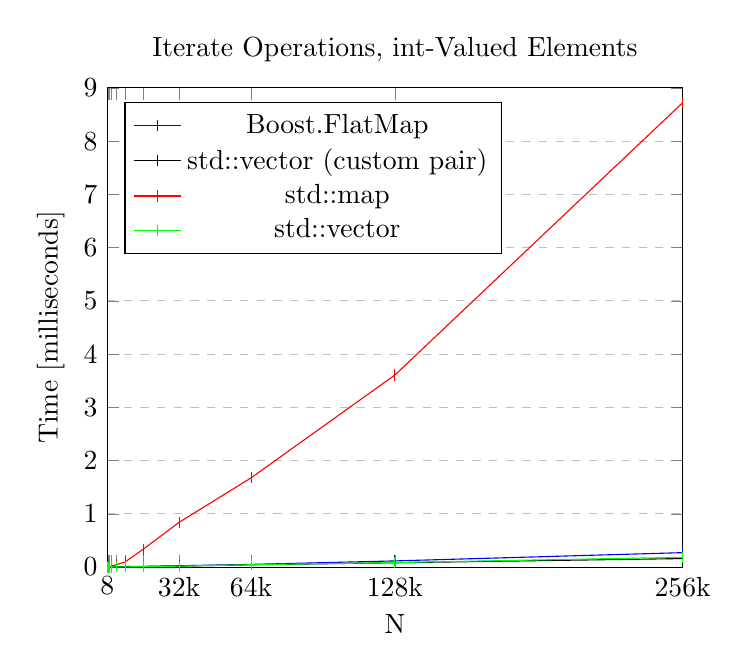
\begin{tikzpicture}
    \begin{axis}[
        width=3.5in,
        title={Iterate Operations, int-Valued Elements},
        xlabel={N},
        ylabel={Time [milliseconds]},
        xmin=0, xmax=262144,
        ymin=0, ymax=9.0,
        xtick={8,16,32,64,128,256,512,1024,2048,4096,8192,16384,32768,65536,131072,262144,524288},
        xticklabels={8,,,,,,,,,,,,32k,64k,128k,256k,512k},
        ytick={0.0,1.0,2.0,3.0,4.0,5.0,6.0,7.0,8.0,9.0,10.0},
        legend pos=north west,
        ymajorgrids=true,
        grid style=dashed,
        scaled x ticks=false,
        scaled y ticks=true,
        legend entries={Boost.FlatMap,std::vector (custom pair),std::map,std::vector},
        ]

    \addplot[color=blue,mark=|,]
        coordinates {(8,6e-05)(16,0)(32,0.00012)(64,0.0001802)(128,0.0001804)(256,6e-05)(512,0.0003606)(1024,0.000601)(2048,0.0014424)(4096,0.0027042)(8192,0.0096752)(16384,0.0132206)(32768,0.0251192)(65536,0.0502984)(131072,0.115681)(262144,0.270963)};

    \addplot[color=black,mark=|,]
        coordinates {(8,0)(16,0)(32,0)(64,0.0001204)(128,6e-05)(256,0)(512,0.000301)(1024,0.000361)(2048,0.0008412)(4096,0.0022834)(8192,0.0033052)(16384,0.0081726)(32768,0.0181482)(65536,0.0431476)(131072,0.0811268)(262144,0.15991)};

    \addplot[color=red,mark=|,]
        coordinates {(8,0)(16,0.00018)(32,0.0003006)(64,0.0004208)(128,0.0008416)(256,0.0015626)(512,0.0087738)(1024,0.0120788)(2048,0.01923)(4096,0.0427268)(8192,0.0970516)(16384,0.334482)(32768,0.840593)(65536,1.67548)(131072,3.60768)(262144,8.72082)};

    \addplot[color=green,mark=|,]
        coordinates {(8,0)(16,6e-05)(32,0.00012)(64,6e-05)(128,0.00024)(256,0.00012)(512,0.0003006)(1024,0.000541)(2048,0.0010216)(4096,0.0029448)(8192,0.0034856)(16384,0.008954)(32768,0.0174874)(65536,0.0441088)(131072,0.0848524)(262144,0.183527)};

    \end{axis}
\end{tikzpicture}
\end{center}


For all variants but \code{map}, iteration is relatively similar, and much
faster that \code{map}'s.

\begin{center}
    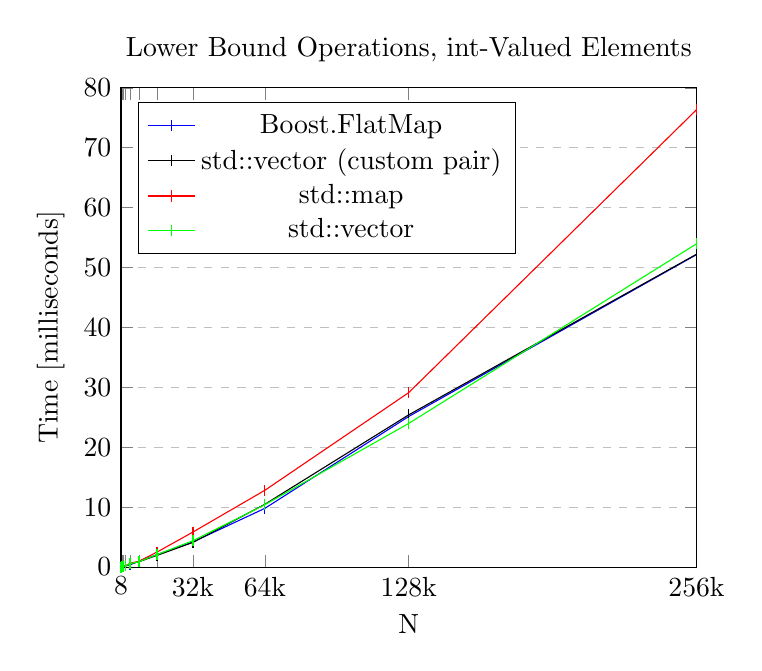
\begin{tikzpicture}
    \begin{axis}[
        width=3.5in,
        title={Lower Bound Operations, int-Valued Elements},
        xlabel={N},
        ylabel={Time [milliseconds]},
        xmin=0, xmax=262144,
        ymin=0, ymax=80.0,
        xtick={8,16,32,64,128,256,512,1024,2048,4096,8192,16384,32768,65536,131072,262144,524288},
        xticklabels={8,,,,,,,,,,,,32k,64k,128k,256k,512k},
        ytick={0.0,10.0,20.0,30.0,40.0,50.0,60.0,70.0,80.0,90.0},
        legend pos=north west,
        ymajorgrids=true,
        grid style=dashed,
        scaled x ticks=false,
        scaled y ticks=true,
        legend entries={Boost.FlatMap,std::vector (custom pair),std::map,std::vector},
        ]

    \addplot[color=blue,mark=|,]
        coordinates {(8,0.0004206)(16,0.0008416)(32,0.002464)(64,0.0042664)(128,0.009135)(256,0.0207914)(512,0.0438094)(1024,0.0908068)(2048,0.191705)(4096,0.385146)(8192,0.977662)(16384,2.07847)(32768,4.19496)(65536,9.80565)(131072,25.1402)(262144,52.158)};

    \addplot[color=black,mark=|,]
        coordinates {(8,0.0003006)(16,0.0009616)(32,0.002524)(64,0.004808)(128,0.0106356)(256,0.021934)(512,0.0477766)(1024,0.0954882)(2048,0.199747)(4096,0.541513)(8192,0.896534)(16384,1.95016)(32768,4.12034)(65536,10.4824)(131072,25.4174)(262144,52.2255)};

    \addplot[color=red,mark=|,]
        coordinates {(8,0.0005408)(16,0.0011424)(32,0.0016226)(64,0.0036058)(128,0.0097956)(256,0.019951)(512,0.0710902)(1024,0.105765)(2048,0.196082)(4096,0.62353)(8192,0.977013)(16384,2.50079)(32768,5.8489)(65536,12.8191)(131072,29.1284)(262144,76.3457)};

    \addplot[color=green,mark=|,]
        coordinates {(8,0.000421)(16,0.0010812)(32,0.003245)(64,0.0048678)(128,0.0109984)(256,0.0224162)(512,0.0484954)(1024,0.101079)(2048,0.207146)(4096,0.565718)(8192,0.899787)(16384,2.08118)(32768,4.39972)(65536,10.4167)(131072,23.987)(262144,53.9652)};

    \end{axis}
\end{tikzpicture}
\end{center}


\code{lower_bound()} performance is roughly similar across all the
implementations, and they all show superlinear growth.  Note that
Boost.FlatMap performs the best here.

\begin{center}
    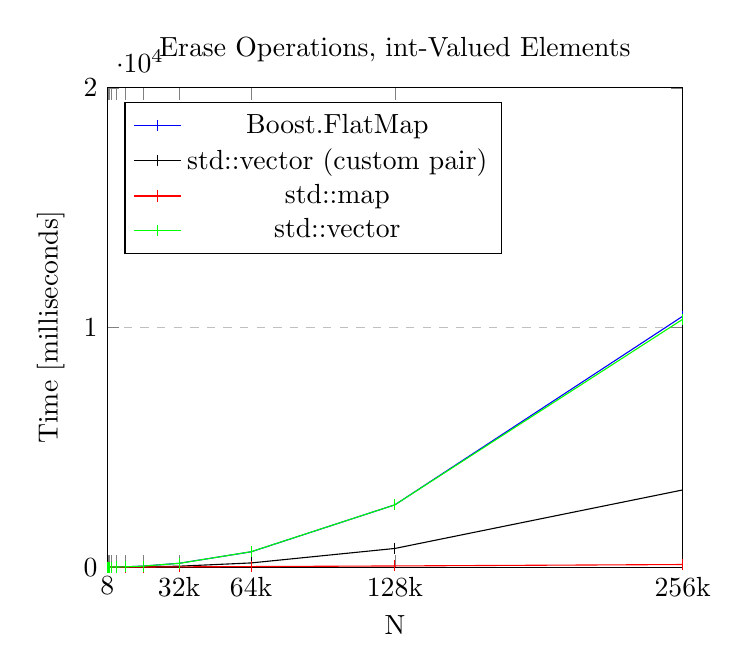
\begin{tikzpicture}
    \begin{axis}[
        width=3.5in,
        title={Erase Operations, int-Valued Elements},
        xlabel={N},
        ylabel={Time [milliseconds]},
        xmin=0, xmax=262144,
        ymin=0, ymax=20000.0,
        xtick={8,16,32,64,128,256,512,1024,2048,4096,8192,16384,32768,65536,131072,262144,524288},
        xticklabels={8,,,,,,,,,,,,32k,64k,128k,256k,512k},
        ytick={0.0,10000.0,20000.0,30000.0},
        legend pos=north west,
        ymajorgrids=true,
        grid style=dashed,
        scaled x ticks=false,
        scaled y ticks=true,
        legend entries={Boost.FlatMap,std::vector (custom pair),std::map,std::vector},
        ]

    \addplot[color=blue,mark=|,]
        coordinates {(8,0.0003604)(16,0.0015022)(32,0.0027644)(64,0.0055284)(128,0.0129792)(256,0.0307674)(512,0.0858164)(1024,0.240433)(2048,0.772987)(4096,2.59798)(8192,10.7093)(16384,42.9557)(32768,158.977)(65536,637.66)(131072,2599.47)(262144,10468.1)};

    \addplot[color=black,mark=|,]
        coordinates {(8,0.0003608)(16,0.0009008)(32,0.002224)(64,0.0045666)(128,0.0101556)(256,0.0240972)(512,0.0510204)(1024,0.118262)(2048,0.292477)(4096,0.877491)(8192,2.67778)(16384,10.2989)(32768,37.8293)(65536,173.616)(131072,778.332)(262144,3219.09)};

    \addplot[color=red,mark=|,]
        coordinates {(8,0.000721)(16,0.0021034)(32,0.0038464)(64,0.0105168)(128,0.0153844)(256,0.0366574)(512,0.132332)(1024,0.185631)(2048,0.386164)(4096,0.989028)(8192,1.82385)(16384,4.31049)(32768,9.85084)(65536,21.7539)(131072,47.844)(262144,107.44)};

    \addplot[color=green,mark=|,]
        coordinates {(8,0.000481)(16,0.001142)(32,0.0026442)(64,0.004988)(128,0.012198)(256,0.030949)(512,0.081968)(1024,0.291638)(2048,0.721907)(4096,3.36513)(8192,10.388)(16384,41.5919)(32768,156.09)(65536,641.439)(131072,2600.19)(262144,10341.3)};

    \end{axis}
\end{tikzpicture}
\end{center}


Erasure has a similar performance profile to insertion, except that the sorted
\code{vector<pair<int, int>>} performs substantially better than
Boost.FlatMap.\\


\subsection{Implications}

TODO Iteration is vastly cheaper for contiguous-storage variants.  It has been
suggested that a \code{map} with a custom allocator can achieve similar
performance to flat data structures, but this would not apply to iteration
performance, unless the values were added to the \code{map} in sorted order.\\

In all the graphs above, the reason the custom-\code{pair} sorted vector
performs so much better than \code{vector<pair<int, int>>} seems to be that
the custom-\code{pair} type has \code{nothrow} special functions.
Implementing all the special functions and adding \code{nothrow(false)} to
each makes the custom-\code{pair} version perform identically to the
\code{pair<int, int>} version.

Boost.FlatMap differs quite a bit from a sorted \code{vector}.  Clearly there
are a lot of QOI choices to make in implementing a standard \code{flat_map}.
